
%(BEGIN_QUESTION)
% Copyright 2012, Tony R. Kuphaldt, released under the Creative Commons Attribution License (v 1.0)
% This means you may do almost anything with this work of mine, so long as you give me proper credit

This hydrostatic liquid level transmitter system has been equipped with {\it standpipes} and extra hand valves to enable ``wet calibration'' of the transmitter:

$$\includegraphics[width=15.5cm]{i01016x01.eps}$$

First, identify the proper position ({\it open} or {\it shut}) for each hand valve when the transmitter is in regular operation.

\vskip 10pt

Next, specify a procedure to apply an LRV ``test pressure'' to the transmitter using the valves and standpipe(s).

\underbar{file i01016}
%(END_QUESTION)





%(BEGIN_ANSWER)

During regular operation: 
 
\begin{itemize}
\item{} Open valves: 2, 4, 5, and 8
\item{} Shut valves: 1, 3, 6, 7, and 9
\end{itemize}

\vskip 10pt

Procedure to apply an LRV test pressure to the transmitter:

\begin{itemize}
\item{} Shut valves 2 and 4
\item{} Open valves 1 and 6
\item{} Inspect wet-leg liquid level (re-fill if necessary)
\item{} Crack valve 4 open until liquid overflows out of LRV standpipe, then shut
\item{} {\it The transmitter will now be sensing LRV pressure}
\end{itemize}

%(END_ANSWER)





%(BEGIN_NOTES)



%INDEX% Calibration, generating LRV and URV for hydrostatic transmitter using standpipes
%INDEX% Measurement, level: hydrostatic pressure

%(END_NOTES)


